% Solutions to the exercises of Chapter 1. Numbers: code/solutions/sol01.py
\documentclass[../solutions_manual.tex]{subfiles}
\begin{document}
\ifSubfilesClassLoaded{\setcounter{chapter}{0}}{}% NN-1 when built standalone
\setcounter{chapter}{0}% NN-1, so this chapter is numbered NN
\chapter{Economics in Matrix Notation}\label{sol01}
\sloppy

All numbers below are printed by \texttt{python3 code/solutions/sol01.py}.

%% ---------------------------------------------------------------------
\exercisesolution{1.1}{Reading the allocation matrix}

\solpart{a} Agent~3's bundle is row~3 of $X$: $x_3 = (1, 1, 5)'$, one unit of Food, one of Clothing and five of Housing.

What she is ``good at'' cannot be read off $X$. The allocation matrix records \emph{consumption} (Definition~\ref{ch01:def:allocation}); production and endowments are in $\Omega$. After trade, consumption reflects preferences and wealth, not what an agent brings to the market: in the Cobb--Douglas example of Section~\ref{ch01:sec:consumer}, Ana (a farmer) and Boris (a tailor) end up with identical bundles. The inference ``she consumes housing, so she produces housing'' is valid only under autarky ($W = I$, $X = \Omega$). With that caveat, a strong answer says: if there were no trade, agent~3 would be a housing producer (a builder or landlord); with trade, her bundle says only that she spends about $5/7 = 0.7143$ of her consumption on housing, much more than anyone else.

\emph{Common mistake:} treating a row of $X$ as a row of $\Omega$.

\solpart{b} Total housing is the third entry of $\ones'X$: $1 + 2 + 5 + 2 = 10$. Agent~3 consumes the most housing (5 units, half the total).

\solpart{c} $\ones'X = (5+2+1+4,\ 3+4+1+2,\ 1+2+5+2) = (12, 10, 10) = \ones'\Omega$. The allocation is feasible with equality (no waste), Definition~\ref{ch01:def:feasibility}.

\solpart{d} The rank of $X$ is $3 = \min(N, L)$, the largest possible. Rows~1--3 alone are linearly independent: their determinant is
\[
\det\begin{pmatrix} 5 & 3 & 1 \\ 2 & 4 & 2 \\ 1 & 1 & 5 \end{pmatrix} = 64 \neq 0 .
\]
So yes: in the sense of the Key Insight of Section~\ref{ch01:sec:consumer}, the economy is structurally differentiated. Rows are not proportional, so agents differ in \emph{what} they consume, not only in how much. The budget shares by row are $(0.5556, 0.3333, 0.1111)$, $(0.25, 0.5, 0.25)$, $(0.1429, 0.1429, 0.7143)$ and $(0.5, 0.25, 0.25)$. Under identical Cobb--Douglas preferences all four rows would be equal and $X$ would have rank one (equation~\eqref{ch01:eq:CD_matrix}).

Rank is a coarse measure: almost every real matrix has full rank. The singular values are a finer one. Here they are $(9.3515, 4.2242, 2.1694)$, so the best rank-one approximation captures $9.3515^2/\sum_k\sigma_k^2 = 0.7950$ of $\|X\|_F^2$. About 80\% of the matrix is ``same bundle, different scale''; the rest is differentiation.

%% ---------------------------------------------------------------------
\exercisesolution{1.2}{Cobb-Douglas equilibrium}

\solpart{a} Agent $i$ maximizes $\frac13\ln x_{i1} + \frac23\ln x_{i2}$ (a monotone transform of $U_i$) subject to $p_1x_{i1} + p_2x_{i2} = w_i$, $w_i = p'\omega_i$; the budget binds because $U_i$ is strictly increasing. The Lagrangian conditions are $\frac{1}{3x_{i1}} = \mu p_1$ and $\frac{2}{3x_{i2}} = \mu p_2$, so $p_1x_{i1} = \frac{1}{3\mu}$ and $p_2x_{i2} = \frac{2}{3\mu}$. Adding them, $w_i = 1/\mu$, hence
\[
x_{i1}^* = \frac{w_i}{3p_1}, \qquad x_{i2}^* = \frac{2w_i}{3p_2}.
\]
Each agent spends one third of her wealth on good~1 and two thirds on good~2. The solution is interior (log utility goes to $-\infty$ at the boundary), and the objective is strictly concave, so this is the unique maximizer.

\solpart{b} Totals: $\ones'\Omega = (4+1+3,\ 1+3+2) = (8, 6)$. With $p_1 = 1$, $w_i = \omega_{i1} + p_2\omega_{i2}$ and $\sum_i w_i = 8 + 6p_2$. Market clearing for good~1:
\[
\sum_i \frac{w_i}{3} = 8 \iff \frac{8 + 6p_2}{3} = 8 \iff p_2^* = \frac{16}{6} = \frac{8}{3} \approx 2.6667.
\]
By Walras' law, $p'z(p) = 0$ for every $p$, where $z$ is aggregate excess demand (the script checks it at $p_2 = 0.5, 1, 4$), so good~2 clears too. Directly: $\frac{2(8 + 16)}{3 \cdot 8/3} = 6$.

\solpart{c} Wealth at $p^* = (1, 8/3)$: $w = (4 + \frac83,\ 1 + 8,\ 3 + \frac{16}{3}) = (6.6667, 9, 8.3333)$. Then $x_{i1} = w_i/3$ and $x_{i2} = 2w_i/(3 \cdot 8/3) = w_i/4$:
\[
X^* = \begin{pmatrix} 2.2222 & 1.6667 \\ 3.0000 & 2.2500 \\ 2.7778 & 2.0833 \end{pmatrix}, \qquad \ones'X^* = (8, 6) = \ones'\Omega .
\]
Feasible with equality. As in the chapter, $X^* = \w\,(1/3,\ 1/4)$ has rank one: everyone spends the same budget shares $(1/3, 2/3)$, and agents differ only in wealth. Agent~2, whose endowment is rich in the expensive good, is now the richest.

%% ---------------------------------------------------------------------
\exercisesolution{1.3}{Welfare loss computation}

By Proposition~\ref{ch01:prop:welfare_loss}, $L = \frac{\kappa N}{2}\Var(\omega) = 0.25\,\Var(\omega)$ here, with $\Var(\omega) = \frac1N\sum_i\omega_i^2 - 1$ since $\Omega/N = 1$. First-best welfare is $\mathcal{W}^{FB} = 5\,U(1) = 4.75$. The largest endowment in all three cases is 5, and $\kappa\cdot 5 = 0.5 < 1$, so every $U$ is increasing on the relevant range.

\solpart{a} $\boldsymbol\omega = \ones$: $\Var = 0$ and $L = 0$.

\solpart{b} $\frac15(9 + 1 + 0.25 + 0.0625 + 0.0625) = 2.075$, so $\Var = 1.075$ and $L = 0.25 \times 1.075 = 0.26875$. Directly, $\mathcal{W}^{FB} - \sum_i U(\omega_i) = 0.26875$.

\solpart{c} $\frac15 \cdot 25 = 5$, so $\Var = 4$ and $L = 1.0$: about 21\% of first-best welfare is lost when one person holds everything.

\solpart{d} $L$ is \emph{not} a function of the Gini coefficient. We use $G(\boldsymbol\omega) = \frac{1}{2N^2\mu}\sum_{i,j}|\omega_i - \omega_j|$, whose maximum is $(N-1)/N = 0.8$. The three cases have $G = 0$, $0.5$ and $0.8$.
\begin{itemize}
\item \textbf{Along a path.} On the family $\boldsymbol\omega(t) = (1-t)\ones + t\cdot 5e_1$, both measures are explicit: $G = 0.8t$ and $\Var = 4t^2$, so $L = t^2 = 1.5625\,G^2$, a convex curve through $(0.8, 1)$.
\item \textbf{Same Gini, different loss.} $(2, 2, 1, 0, 0)$ and $(3.4, 0.4, 0.4, 0.4, 0.4)$ both have $G = 0.48$, but $L = 0.2$ and $L = 0.36$. Gini weights absolute differences; $L$ weights squared deviations, so it penalizes one very rich agent more.
\item \textbf{A bound that always holds.} By Cauchy--Schwarz, $\frac{1}{N^2}\sum_{i,j}|\omega_i - \omega_j| \le \bigl(\frac{1}{N^2}\sum_{i,j}(\omega_i-\omega_j)^2\bigr)^{1/2} = \sqrt{2\Var}$. Hence $2\mu G \le \sqrt{2\Var}$, i.e.\ $\Var \ge 2\mu^2G^2$ and
\[
L \ \ge\ \kappa N\mu^2 G^2 = 0.5\,G^2 .
\]
\item \textbf{A sample.} The script draws 20{,}000 random endowment vectors (Dirichlet, scaled to $\Omega = 5$). All satisfy the bound. For $G \in [0.39, 0.41)$, $L$ ranges over $[0.1200, 0.2315]$; for $G \in [0.59, 0.61)$, over $[0.3142, 0.5366]$.
\end{itemize}

\begin{center}
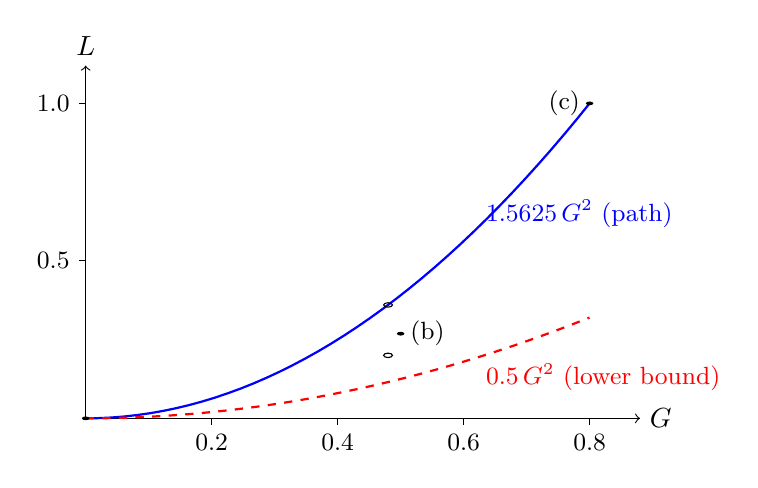
\begin{tikzpicture}[x=8cm,y=4cm]
\draw[->] (0,0) -- (0.88,0) node[right] {$G$};
\draw[->] (0,0) -- (0,1.12) node[above] {$L$};
\foreach \g in {0.2,0.4,0.6,0.8} \draw (\g,0) -- (\g,-0.02) node[below] {\small\g};
\foreach \l in {0.5,1.0} \draw (0,\l) -- (-0.01,\l) node[left] {\small\l};
\draw[thick,blue] plot[domain=0:0.8,samples=40] (\x,{1.5625*\x*\x});
\draw[thick,dashed,red] plot[domain=0:0.8,samples=40] (\x,{0.5*\x*\x});
\fill (0,0) circle (0.006) (0.5,0.26875) circle (0.006) (0.8,1.0) circle (0.006);
\node[right] at (0.5,0.26875) {\small (b)};
\node[left] at (0.8,1.0) {\small (c)};
\draw (0.48,0.2) circle (0.007) (0.48,0.36) circle (0.007);
\node[blue,right] at (0.62,0.65) {\small $1.5625\,G^2$ (path)};
\node[red,right] at (0.62,0.13) {\small $0.5\,G^2$ (lower bound)};
\end{tikzpicture}
\end{center}

\emph{Model answer.} The welfare cost of inequality with quadratic utility is a variance, not a Gini. Two economies with the same Gini can have different losses, and $L$ grows at least quadratically in $G$. \emph{Common mistake:} plotting one point per Gini value, as if $L(G)$ were a function.

%% ---------------------------------------------------------------------
\exercisesolution{1.4}{Bargaining with different power}

The surplus is $\Omega - \sum_j d_j = 2 - 0.8 = 1.2$, and $U(x) = x - 0.25x^2$.

\solpart{a} The utilitarian planner equalizes marginal utilities $1 - \kappa x_i$ (Example~\ref{ch01:ex:one_good}), so $x^{FB} = (1, 1)$, $U = (0.75, 0.75)$ and $\mathcal{W}^{FB} = 1.5$. Both agents get more than their disagreement payoffs, so the first-best is also individually rational.

\solpart{b} By Proposition~\ref{ch01:prop:nash_division}, $x_i = d_i + \lambda_i\cdot 1.2$. With $\boldsymbol\lambda = (0.5, 0.5)$: $x = (1.2, 0.8)$, $U = (0.84, 0.64)$ and $\mathcal{W} = 1.48$. The loss relative to the first-best is $0.02$. Because $U$ is quadratic and $\sum_i(x_i - 1) = 0$, the loss is exactly $\frac{\kappa}{2}\sum_i(x_i - 1)^2 = 0.25(0.04 + 0.04) = 0.02$, the same computation as in the proof of Proposition~\ref{ch01:prop:allocation_rule}. Equal power does not give equal division, because outside options differ.

\solpart{c} With $\boldsymbol\lambda = (0.8, 0.2)$: $x = (0.6 + 0.96,\ 0.2 + 0.24) = (1.56, 0.44)$, $U = (0.9516, 0.3916)$, $\mathcal{W} = 1.3432$, and the loss is $0.1568 = 0.25(0.3136 + 0.3136)$. Agent~1 benefits: she gains $0.1116$ in utility over equal power, and agent~2 loses $0.2484$. Both still beat disagreement ($U(d) = (0.51, 0.19)$), and $\kappa x = (0.78, 0.22) < 1$, so the allocation is Pareto efficient (Proposition~\ref{ch01:prop:nash_division}). The loss is distributional, not an inefficiency.

\solpart{d} Solve $d_i + \lambda_i \cdot 1.2 = 1$: $\boldsymbol\lambda^* = \bigl(\frac{0.4}{1.2}, \frac{0.8}{1.2}\bigr) = (0.3333, 0.6667)$. It sums to one because $\sum_i(1 - d_i) = 2 - 0.8 = 1.2$. As in Example~\ref{ch01:ex:bargaining}, reaching the first-best requires giving \emph{more} power to the agent with the worse outside option.

%% ---------------------------------------------------------------------
\exercisesolution{1.5}{The cascade in action}

\solpart{a} $A' = \begin{pmatrix} 0.2 & 0.3 \\ 0.1 & 0.1\end{pmatrix}$, and
\[
(A')^2 = \begin{pmatrix} 0.07 & 0.09 \\ 0.03 & 0.04 \end{pmatrix},\quad
(A')^3 = \begin{pmatrix} 0.023 & 0.030 \\ 0.010 & 0.013 \end{pmatrix},\quad
(A')^4 = \begin{pmatrix} 0.0076 & 0.0099 \\ 0.0033 & 0.0043 \end{pmatrix}.
\]
For example, $(A')^2_{11} = 0.2\cdot0.2 + 0.3\cdot0.1 = 0.07$. Each round is roughly a third of the previous one, the rate $\rho(A)$ of part~(c).

\solpart{b} $S_4 = \sum_{k=0}^4(A')^k = \begin{pmatrix} 1.3006 & 0.4299 \\ 0.1433 & 1.1573\end{pmatrix}$. The exact inverse is $\det(I - A') = 0.8\cdot0.9 - 0.3\cdot0.1 = 0.69$ and
\[
(I - A')^{-1} = \frac{1}{0.69}\begin{pmatrix} 0.9 & 0.3 \\ 0.1 & 0.8\end{pmatrix} = \begin{pmatrix} 1.3043 & 0.4348 \\ 0.1449 & 1.1594\end{pmatrix}.
\]
The error is $L - S_4 = \begin{pmatrix} 0.0037 & 0.0049 \\ 0.0016 & 0.0021\end{pmatrix}$, i.e.\ relative errors from $0.18\%$ to $1.12\%$; the off-diagonal entries converge slowest because they need at least one indirect round. The error has an exact form: telescoping (Appendix~\ref{ch01:app:neumann}) gives $L - S_K = (A')^{K+1}L$, which the script confirms for $K = 4$. The error is nonnegative and shrinks geometrically.

\solpart{c} Appendix~\ref{ch01:app:spectral_radius}: trace $0.3$ and determinant $0.02 - 0.03 = -0.01$, so $\lambda = (0.3 \pm \sqrt{0.13})/2 = (0.3 \pm 0.36056)/2$, giving $\lambda_1 = 0.33028$ and $\lambda_2 = -0.03028$. Then $\rho(A) = 0.33028 < 1$. Sanity check: $\rho(A)$ is at most the largest row sum, $0.4$.

\solpart{d} The output multipliers are the column sums of $L$: $(1.4493, 1.5942)$. Sector~2 has the stronger backward linkages. The reason is in the recipes: sector~2 needs $0.3 + 0.1 = 0.4$ of inputs per unit, sector~1 only $0.3$, and sector~2's main input (good~1, $a_{21} = 0.3$) is itself input-intensive. The forward linkages (row sums of $L$) are $(1.7391, 1.3043)$: good~1 is the more widely used input. Both vectors have the same mean, $1.5217$, as they must.

%% ---------------------------------------------------------------------
\exercisesolution{1.6}{Properties of $W^{CE}$}

\solpart{a} $\ones'\ones = N$, so $(W^{CE})^2 = \frac{1}{N^2}\ones(\ones'\ones)\ones' = \frac{N}{N^2}\ones\ones' = W^{CE}$. $W^{CE}$ is the orthogonal projection onto $\operatorname{span}(\ones)$.

\solpart{b} $(W^{CE}\x)_i = \sum_j \frac1N x_j = \bar x$ for every $i$, so $W^{CE}\x = \bar x\ones$. \emph{Interpretation:} one round of anonymous interaction replaces every individual value (a belief, a price signal, an endowment-weighted demand) by the population mean. Individual identity is erased in a single step. This is the ``anonymous'' property~(a) of Section~\ref{ch01:sec:implicit_W}.

\solpart{c} $W^{CE}\ones = \ones$ by (b), since $\bar 1 = 1$. If $\ones'\x = 0$ then $W^{CE}\x = \bar x\ones = 0$, so the subspace $\ones^\perp$, of dimension $N-1$, consists of eigenvectors with eigenvalue 0. $\R^N = \operatorname{span}(\ones) \oplus \ones^\perp$, so the geometric multiplicities add to $N$ and there are no other eigenvalues. Since $W^{CE}$ is symmetric, the algebraic and geometric multiplicities agree; equivalently, its characteristic polynomial is $\lambda^{N-1}(\lambda - 1)$. For $N = 3$, a basis of the eigenspace for 0 is $(1, -1, 0)'$, $(1, 0, -1)'$; an orthonormal one is $(1,-1,0)'/\sqrt2$, $(1,1,-2)'/\sqrt6$.

\solpart{d} $W = \begin{pmatrix} 0.3333 & 0.3333 & 0.3333 \\ 0.6667 & 0.1667 & 0.1667 \\ 0 & 0.5 & 0.5\end{pmatrix}$. Row sums $(1,1,1)$; column sums $\frac13(3, 3, 3) = (1, 1, 1)$. So \emph{yes}, $W$ is doubly stochastic, and by Proposition~\ref{ch01:prop:pi_uniform} $\boldsymbol\pi = \frac13\ones$.

With $\x = (3, 6, 9)'$: $W\x = (6, 4.5, 7.5)'$, while $W^{CE}\x = (6, 6, 6)'$. What is different:
\begin{itemize}
\item \textbf{Non-anonymity.} $W$ preserves the mean ($\ones'W\x = 18 = \ones'\x$, because columns sum to one) but not the identity of who listens to whom. Agent~2 puts $2/3$ of her weight on agent~1 and moves to $4.5$; agent~3 ignores agent~1 and moves to $7.5$.
\item \textbf{Same coordinates, different matrix.} $W$ has rank~2 (columns~2 and~3 are equal), and its eigenvalues are $\{1, 0, 0\}$: trace~1 and determinant~0 force the other two to sum to 0 and multiply to 0. So $\Gamma(W) = 1$, as for $W^{CE}$. But $0$ has algebraic multiplicity 2 and geometric multiplicity 1, so $W - W^{CE}$ is a nonzero nilpotent matrix with $(W - W^{CE})^2 = 0$. Hence $W^2 = W^{CE}$ exactly (use $WW^{CE} = W^{CE}W = W^{CE}$), and $W^2\x = (6,6,6)'$.
\end{itemize}
\emph{Lesson:} the two coordinates of Section~\ref{ch01:sec:conventions} (power $\boldsymbol\pi$ and integration $\Gamma$) are identical for $W$ and $W^{CE}$, yet the matrices differ in what happens along the way. Uniform power does not imply anonymity.

%% ---------------------------------------------------------------------
\exercisesolution{1.7}{Bolivia's input-output table (data exercise)}

\textbf{Data (real results).} INE Bolivia, supply-use tables, base 2017, year 2019 \citep{ine2026sut}, retrieved 2026-11-05. The repository converts them to an industry-by-industry table of \emph{domestic} flows at basic prices (\texttt{data/compute/compute\_bolivia\_io.py}: purchasers' to basic prices, import proportionality, fixed product-sales structure) and aggregates it to the book's 12 sectors (\texttt{data/processed/bolivia\_Z/Z\_2017\_2019\_book12.csv}, millions of current Bs). Gross output comes from \texttt{data/processed/bolivia\_io\_sector\_facts.csv}. We aggregate further to six sectors: Hydrocarbons, Mining, Agriculture, Manufacturing (which includes refining), Construction, and Services (the remaining seven sectors). Gross output, in million Bs: $25{,}863$; $25{,}009$; $46{,}473$; $114{,}506$; $51{,}045$; $287{,}812$.

\solpart{a} Published flows have rows = sellers: $Z_{s s'}$ is the sales of $s$ to $s'$. In the book's convention, $a_{ij} = Z_{ji}/x_i$ (the purchases of $i$ from $j$ per unit of $i$'s output), i.e.\ $A = (Z\,\text{diag}(\x)^{-1})'$:
\[
A = \begin{pmatrix}
0.0056 & 0.0017 & 0.0009 & 0.0131 & 0.0015 & 0.2019\\
0.0043 & 0.0009 & 0.0042 & 0.0567 & 0.0017 & 0.1700\\
0.0047 & 0.0013 & 0.1171 & 0.0641 & 0.0067 & 0.1601\\
0.0357 & 0.1121 & 0.1922 & 0.1091 & 0.0027 & 0.1059\\
0.0005 & 0.0313 & 0.0010 & 0.2045 & 0.0380 & 0.0632\\
0.0093 & 0.0010 & 0.0109 & 0.0646 & 0.0076 & 0.1811
\end{pmatrix}
\]
(rows and columns in the order above). The row sums are the domestic intermediate inputs per unit of output: $(0.2246, 0.2378, 0.3540, 0.5576, 0.3385, 0.2746)$. They match the INE-derived figures quoted in Chapter~3 (hydrocarbons $0.225$, manufacturing $0.558$). $\rho(A) = 0.3473 < 1$, so the economy is productive.

\solpart{b} $L = (I - A')^{-1}$:
\[
L = \begin{pmatrix}
1.0094 & 0.0096 & 0.0116 & 0.0460 & 0.0116 & 0.0154\\
0.0061 & 1.0107 & 0.0138 & 0.1320 & 0.0618 & 0.0125\\
0.0120 & 0.0259 & 1.1586 & 0.2582 & 0.0594 & 0.0365\\
0.0356 & 0.0838 & 0.1046 & 1.1693 & 0.2578 & 0.0965\\
0.0038 & 0.0040 & 0.0104 & 0.0073 & 1.0419 & 0.0105\\
0.2574 & 0.2284 & 0.2466 & 0.2410 & 0.1410 & 1.2480
\end{pmatrix}.
\]

\solpart{c} The output multipliers (column sums of $L$) are: Hydrocarbons $1.324$, Mining $1.363$, Agriculture $1.546$, Manufacturing $1.854$, Construction $1.573$, Services $1.419$. With Mining and Gas merged into one sector, the five-sector multipliers are: Mining/Gas $1.343$, Agriculture $1.546$, Manufacturing $1.852$, Services $1.419$ (Construction $1.572$). Sanity check: mean backward linkage equals mean forward linkage ($1.5132$).

\solpart{d} The highest multiplier is Manufacturing ($1.854$); the lowest is Hydrocarbons ($1.324$), with Mining close behind. On Pinto's question, the measured table does \emph{not} show a block-diagonal $A$. Take the extractive block $\{$Hydrocarbons, Mining$\}$ against the rest. The cross-block mass is $\chi(A) = 0.3250$ (Definition~\ref{ch03:def:heterogeneity}), and the six-sector $\Gamma(W^P) = 0.7467$, with $\Neff = 2.843$ of 6 and $\pi_{\text{Services}} = 0.527$. The extractive sectors buy 97.29\% of their domestic intermediate inputs from the rest of the economy (mostly services), and the rest buys 12.34\% of its domestic inputs from them. Bolivia's heterogeneity lies elsewhere: in how \emph{little} the extractive sectors buy domestically per unit of output ($0.22$--$0.24$, against $0.56$ in manufacturing) and in where their output goes (part~(e)). This matches the measured values in Chapter~3, Section~\ref{ch03:sec:heterogeneity}.

\solpart{e} \textit{Challenge.} The gas sector is an enclave in two precise senses, but not in the sense of zero linkages.
\begin{itemize}
\item \textbf{Backward.} One unit of final demand for hydrocarbons generates $L e_{\text{hyd}} = (1.0094, 0.0061, 0.0120, 0.0356, 0.0038, 0.2574)'$. That is $0.315$ of output in other sectors, almost all of it in services: the lowest spillover of the six sectors (manufacturing: $0.685$).
\item \textbf{Forward.} Its forward linkage is $1.104$, the second lowest, because 70.1\% of its output is exported rather than sold to domestic users.
\item \textbf{Income.} Compensation of employees is 5.95\% of its value added, so the rents reach households through the fiscal system rather than through wages or input purchases (Chapter~3, Section~\ref{ch03:sec:multi_sector}).
\end{itemize}
In the production reading, its Perron weight is $\pi_{\text{hyd}} = 0.0357$ at six sectors (against $1/6$ if uniform). Answer: an export enclave with thin domestic backward and forward linkages, connected to the rest of the economy mainly through services purchases and taxes.

\emph{Caveats.} (i) Domestic flows depend on the import-proportionality assumption, because the SUT does not split domestic from imported use. (ii) Multipliers depend on aggregation: the 12-sector values in \texttt{data/processed/bolivia\_io\_linkages.csv} differ slightly. (iii) \emph{Common mistake:} computing multipliers from $W^P$. For any row-stochastic $W$, $(I - \gamma W)^{-1}\ones = \ones/(1-\gamma)$, so every row-sum linkage is identical (Section~\ref{ch01:sec:conventions}).

%% ---------------------------------------------------------------------
\exercisesolution{1.8}{From story to matrix}

\solpart{a} The agents are 1 Mar\'ia, 2 Wholesaler, 3 Sugar Shop, 4 Cinnamon Distributor, 5 Charcoal Supplier. Following the book's convention (Appendix~\ref{ch05:app:graphs}), draw $i \to j$ when $i$ uses $j$'s output; influence and demand impulses flow against the arrows.
\begin{center}
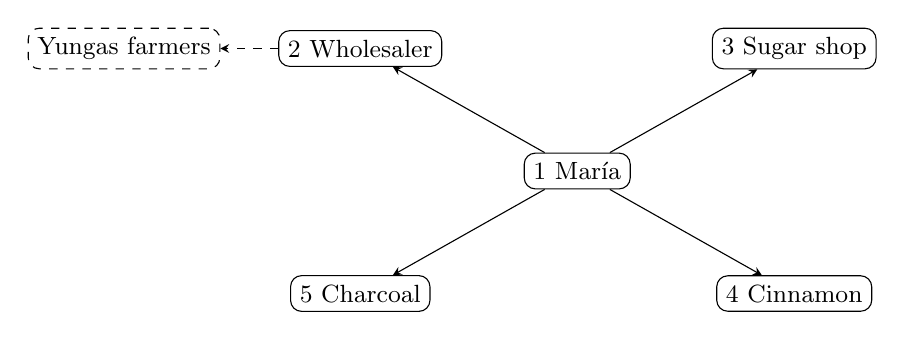
\begin{tikzpicture}[node distance=2.2cm,>=stealth,every node/.style={draw,rounded corners,font=\small}]
\node (M) {1 Mar\'ia};
\node (W) [above left of=M,xshift=-1.2cm] {2 Wholesaler};
\node (S) [above right of=M,xshift=1.2cm] {3 Sugar shop};
\node (C) [below right of=M,xshift=1.2cm] {4 Cinnamon};
\node (H) [below left of=M,xshift=-1.2cm] {5 Charcoal};
\node (Y) [left of=W,xshift=-0.8cm,dashed] {Yungas farmers};
\draw[->] (M) -- (W); \draw[->] (M) -- (S); \draw[->] (M) -- (C); \draw[->] (M) -- (H);
\draw[->,dashed] (W) -- (Y);
\end{tikzpicture}
\end{center}
The Yungas farmers are outside the five-agent system (dashed).

\solpart{b} With $G_{ij} = 1$ if $i$ uses $j$'s output (written $G$ to avoid a clash with the coefficient matrix; Appendix~\ref{ch05:app:graphs}):
\[
G = \begin{pmatrix} 0 & 1 & 1 & 1 & 1\\ 0&0&0&0&0\\ 0&0&0&0&0\\ 0&0&0&0&0\\ 0&0&0&0&0\end{pmatrix}.
\]
The in-degrees (column sums) are $(0, 1, 1, 1, 1)$ and the out-degrees $(4, 0, 0, 0, 0)$.

\solpart{c} $G$ is not symmetric. The asymmetry is the \emph{direction of dependence}: Mar\'ia depends on four suppliers, and none of them depends on her output. A demand shock to api travels to all four, and a shock to any supplier reaches only Mar\'ia. A symmetric matrix would mean mutual dependence: each supplier would buy api as an input.

\solpart{d} After the wholesaler's row and column are set to zero, only Mar\'ia is \emph{directly} affected: $G_{12} = 1$ was the only entry in column~2. For the cascade, note that $G^2 = 0$ (nobody buys from Mar\'ia), so the Neumann series stops after one term: with any coefficient $c$ per link, $(I - cG')^{-1} = I + cG'$. In the demand-driven Leontief model the cascade therefore has depth one. Removing the wholesaler changes the output of agents 3--5 not at all: with $c = 0.25$ and api demand $\mathbf{d} = e_1$, $\y$ goes from $(1, 0.25, 0.25, 0.25, 0.25)$ to $(1, 0, 0.25, 0.25, 0.25)$.

That conclusion is wrong economically, and the reason is instructive. The disappearance of a supplier is a \emph{supply} shock, which travels downstream to users, not upstream like the demand impulses the quantity model $\y = (I - A')^{-1}\mathbf d$ handles (Chapter~3, Section~\ref{ch03:sec:multi_sector}). With fixed proportions and no substitute source of corn, Mar\'ia cannot produce api. Her purchases of sugar, cinnamon and charcoal then fall to zero, so agents~3--5 are \emph{indirectly} affected through her. The Yungas farmers, outside the system, lose their buyer.

\solpart{e} $W^{CE}$ for $N = 5$ has every entry equal to $1/5$: everyone depends equally on everyone, including herself. $G$ has 4 nonzero entries out of 25. It contains exactly the information $W^{CE}$ destroys: \emph{who} depends on \emph{whom} (support), in which \emph{direction} (asymmetry), the hub (Mar\'ia, the only buyer), and the absence of any cycle (nilpotency, hence no feedback). As a weight matrix, $G$ cannot even be row-normalized, because rows 2--5 are zero (the suppliers' own inputs are outside the system). It is reducible, so a Perron vector is not defined until the system is closed. \emph{Common mistake:} treating the binary adjacency matrix as a technical-coefficient matrix with entries 1, for which $\rho(A) < 1$ would fail in any graph with a cycle.

%% ---------------------------------------------------------------------
\exercisesolution{1.9}{From sectors to countries}

\solpart{a} $\rho(A) = 0.1564$. $L = (I - A')^{-1} = \begin{pmatrix} 1.0601 & 0.0118 & 0.0118\\ 0.3534 & 1.0595 & 0.0595\\ 0.3534 & 0.0595 & 1.0595\end{pmatrix}$. The output multipliers (column sums) are $(1.7668, 1.1307, 1.1307)$. Country~1 has by far the strongest backward linkages: its recipe draws $0.30$ from each of the others.

\solpart{b} $L e_2 = (0.0118, 1.0595, 0.0595)'$: a unit of final demand in Country~2 generates $1.0595$ in Country~2, $0.0595$ in Country~3 and only $0.0118$ in Country~1, a total of $1.1307$. By contrast, a unit in Country~1 generates $(1.0601, 0.3534, 0.3534)$, a total of $1.7668$.

\solpart{c} The answer depends on which half of Prebisch's description we look at, and a strong answer says so.
\begin{itemize}
\item \textbf{The demand-pull half matches.} Countries~2 and~3 sell inputs to Country~1 ($a_{12} = a_{13} = 0.30$). Expansion in Country~1 pulls their output ($\ell_{21} = \ell_{31} = 0.3534$), and their own expansion barely reaches Country~1 ($\ell_{12} = 0.0118$). Countries~2 and~3 export primary inputs, and their activity is conditioned by Country~1's demand.
\item \textbf{The import half is reversed.} The periphery imports almost nothing from Country~1 as an input ($a_{21} = a_{31} = 0.01$), whereas in Prebisch the periphery imports manufactures \emph{from} the center.
\end{itemize}
The modification that makes Countries~2 and~3 depend on Country~1's output is
\[
A_{\text{mod}} = \begin{pmatrix} 0.05 & 0.01 & 0.01\\ 0.30 & 0.05 & 0.05\\ 0.30 & 0.05 & 0.05\end{pmatrix} = A'.
\]
Then $L_{\text{mod}} = L'$, and the multipliers become $(1.0836, 1.4723, 1.4723)$: now the periphery has the larger backward linkages (it pulls inputs from the center), and Country~1 has the largest \emph{forward} linkage ($1.7668$).

In the production reading of $\boldsymbol\pi$ (row-normalized $W^P$), Country~1's Perron weight rises from $0.0897$ to $0.7241$. Who is the ``center'' is thus not read from backward linkages alone. The center is the economy whose output others depend on: column sums of $W^P$, $(0.2587, 1.3706, 1.3706)$ before and $(2.2143, 0.3929, 0.3929)$ after.

\solpart{d} \textit{Claim: with a symmetric $A$ there is no center--periphery structure in the linkages.} If $A = A'$, then $L' = ((I - A')^{-1})' = (I - A)^{-1} = L$, so every country's backward linkage (column sum) equals its forward linkage (row sum), and $\ell_{ij} = \ell_{ji}$: an impulse from $i$ to $j$ is as strong as from $j$ to $i$. For example, the symmetric part $(A + A')/2$ gives $\text{BL} = \text{FL} = (1.4995, 1.3694, 1.3694)$. Center--periphery is a statement about \emph{direction} (who conditions whom), so it lives in the antisymmetric part $(A - A')/2$. In the original $A$, $\text{BL} - \text{FL} = (0.6832, -0.3416, -0.3416)$. Asymmetry is necessary but not sufficient: a periphery also needs low weight in others' recipes and a low $\pi$. The rigorous version is Chapter~16's.

\end{document}
